\section{eo\-Plus$<$ EOT $>$ Class Template Reference}
\label{classeo_plus}\index{eoPlus@{eoPlus}}
Very elitist class, copies entire population into next gen.  


{\tt \#include $<$eo\-Merge.h$>$}

Inheritance diagram for eo\-Plus$<$ EOT $>$::\begin{figure}[H]
\begin{center}
\leavevmode
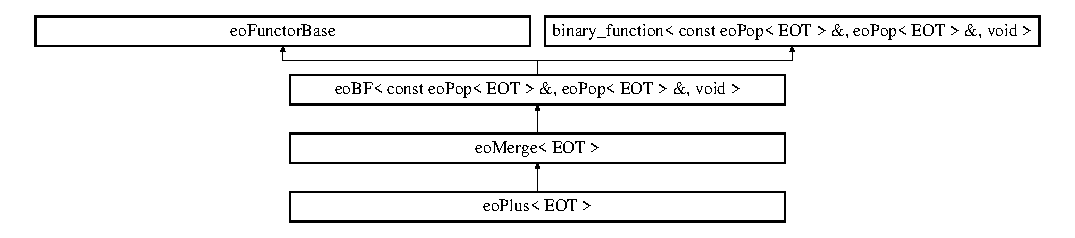
\includegraphics[height=2.75184cm]{classeo_plus}
\end{center}
\end{figure}
\subsection*{Public Member Functions}
\begin{CompactItemize}
\item 
void {\bf operator()} (const {\bf eo\-Pop}$<$ {\bf EOT} $>$ \&\_\-pop, {\bf eo\-Pop}$<$ {\bf EOT} $>$ \&\_\-offspring)\label{classeo_plus_a0}

\begin{CompactList}\small\item\em The pure virtual function that needs to be implemented by the subclass. \item\end{CompactList}\end{CompactItemize}


\subsection{Detailed Description}
\subsubsection*{template$<$class EOT$>$ class eo\-Plus$<$ EOT $>$}

Very elitist class, copies entire population into next gen. 



Definition at line 116 of file eo\-Merge.h.

The documentation for this class was generated from the following file:\begin{CompactItemize}
\item 
eo\-Merge.h\end{CompactItemize}
